\documentclass[12pt]{article}
\usepackage[margin=1in]{geometry} 
\usepackage{amsmath}
\usepackage{amssymb}
\usepackage{siunitx}
\usepackage{float}
\usepackage{tikz}
\def\checkmark{\tikz\fill[scale=0.4](0,.35) -- (.25,0) -- (1,.7) -- (.25,.15) -- cycle;} 
\usepackage{url}
\usepackage[siunitx,american,RPvoltages]{circuitikz}
\ctikzset{capacitors/scale=0.7}
\ctikzset{diodes/scale=0.7}
\usepackage{tabularx}
\newcolumntype{C}{>{\centering\arraybackslash}X}
\renewcommand\tabularxcolumn[1]{m{#1}}% for vertical centering text in X column
\usepackage{tabu}
\usepackage[spanish,es-tabla,activeacute]{babel}
\usepackage{babelbib}
\usepackage{booktabs}
\usepackage{pgfplots}
\usepackage{hyperref}
\hypersetup{colorlinks = true,
            linkcolor = black,
            urlcolor  = blue,
            citecolor = blue,
            anchorcolor = blue}
\usepgfplotslibrary{units, fillbetween} 
\pgfplotsset{compat=1.16}
\usepackage{bm}
\usetikzlibrary{arrows, arrows.meta, shapes, 3d, perspective, positioning}
\renewcommand{\sin}{\sen} %change from sin to sen
\usepackage{bohr}
\setbohr{distribution-method = quantum,insert-missing = true}
\usepackage{elements}
\usepackage{verbatim}
\usetikzlibrary{mindmap,trees,backgrounds}
 
\definecolor{color_mate}{RGB}{255,255,128}
\definecolor{color_plas}{RGB}{255,128,255}
\definecolor{color_text}{RGB}{128,255,255}
\definecolor{color_petr}{RGB}{255,192,192}
\definecolor{color_made}{RGB}{192,255,192}
\definecolor{color_meta}{RGB}{192,192,255}
\usepackage[edges]{forest}
\usepackage{etoolbox}
\usepackage{schemata}
\newcommand\diagram[2]{\schema{\schemabox{#1}}{\schemabox{#2}}}
\usepackage{lastpage}
\usepackage{fancyhdr}
\usepackage{csvsimple,booktabs}
\pagestyle{fancy}
\setlength{\headheight}{42pt}
\usepackage{caption}
 
\begin{document}
\lhead{Ingeniería Física \\ Escuela de Física \\ Tecnológico de Costa Rica} 
\rhead{Instrumentación II \\ Tarea \#1  \\ Entrega: Semana 3} 
\cfoot{\thepage\ de \pageref{LastPage}}
\setlength{\parindent}{0em}

Usando un Notebook de \href{https://colab.research.google.com/}{Google Colab} realice lo siguiente:

\begin{itemize}
    \item Replique el algoritmo mostrado en la Figura \ref{fig:while} usando Python. Use como valor de \emph{\# de grupo} el numero correspondiente a su grupo.
    \begin{figure}[H]
        \centering
        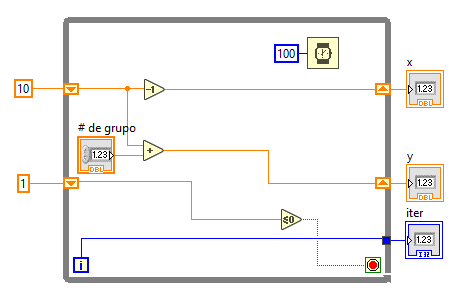
\includegraphics[width=10cm]{fig/t1.1.png}
        \caption{}
        \label{fig:while}
    \end{figure}
    \item Imprima el valor de $x$, $y$ e $iter$ en la terminal una vez terminada la ejecución del bucle While
    \item Descarge el Notebook (.ipynb) y subalo al TecDigital
\end{itemize}

Cualquier entrega tardía se califica en base a 70. 


% \bibliographystyle{IEEEtran}
% \bibliography{ref_tareas}

\end{document}